\documentclass[14pt]{extreport}
\usepackage{indentfirst}
\usepackage[T2A]{fontenc}
\usepackage[utf8]{inputenc}
\usepackage[english,russian]{babel}
\addto\captionsrussian{%
	\renewcommand{\contentsname}{Содержание}%
}
\addto\captionsrussian{%
	\renewcommand{\bibname}{Список литературы}%
}
\usepackage[top = 20mm, left = 30mm, right = 15mm, bottom = 20mm]{geometry}
\setlength\parindent{12.5mm}
\renewcommand{\baselinestretch}{1.5}
\def\hrf#1{\hbox to#1{\hrulefill}}
\usepackage{ragged2e}
\usepackage{caption}
\usepackage{multicol}
\usepackage{mathtools}
\usepackage{url}
\usepackage{xurl}
\usepackage{amsmath,amsfonts,amssymb}
\usepackage{courier}
\usepackage{hyperref}
\usepackage{enumitem}
\usepackage{listings}
\usepackage{xcolor}
\usepackage{courier}
\usepackage{verbatim}
\usepackage{graphicx}
\usepackage{float}

\renewcommand\thesection{\arabic{section}}

% Цвета для подсветки
\definecolor{bluekeywords}{rgb}{0.125,0.375,0.625}
\definecolor{greencomments}{rgb}{0.125,0.5,0.125}
\definecolor{redstrings}{rgb}{0.875,0.125,0.125}
\definecolor{graynumbers}{rgb}{0.5,0.5,0.5}
\definecolor{lightgray}{gray}{0.95}
\definecolor{codegreen}{rgb}{0,0.6,0}
\definecolor{codegray}{rgb}{0.5,0.5,0.5}
\definecolor{codepurple}{rgb}{0.58,0,0.82}
\definecolor{backcolour}{rgb}{0.95,0.95,0.95}

% Макрос для кода (Courier + серый фон)
%\usepackage{tgcursor}  % делает \texttt = TeX Gyre Cursor (аналог Courier)
\newcommand{\code}[1]{\colorbox{lightgray}{\texttt{#1}}}


\lstset{
	language=C++,
	basicstyle=\ttfamily\small,
	keywordstyle=\color{bluekeywords}\bfseries,
	commentstyle=\color{greencomments},
	stringstyle=\color{redstrings},
	numberstyle=\color{graynumbers},
	numbers=left,
	numbersep=10pt,
	columns=fullflexible,
	tabsize=4,
	showspaces=false,
	showstringspaces=false,
	breaklines=true,
	backgroundcolor=\color{lightgray},
	frame=single,
	rulecolor=\color{gray!30!black},
	captionpos=b
}


\begin{document}
	\sloppy
	\thispagestyle{empty}
	\centering{
		Министерство образования и науки Российской Федерации\\
		Федеральное государственное автономное образовательное учреждение высшего образования\\
		«Санкт-Петербургский политехнический университет Петра Великого»\\[10pt]
		Институт компьютерных наук и кибербезопасности\\
		Высшая школа технологий искусственного интеллекта\\
		02.03.01 Математика и компьютерные науки\\
		\vspace{\fill}
		{\large
			Отчёт по дисциплине\\
			{\Large \bf Теоретические основы баз данных\\Курсовая работа}\\
			{\Large <<Каталог объектов дальнего космоса>>}
			\vspace{\fill}
		}

        \centering

\begin{tabular}{|c|c|}
\hline
Часть работы & Подпись преподавателя \\
\hline
Часть I &  \\
\hline
Часть II &  \\
\hline
Часть III &  \\
\hline
\end{tabular}
		
		\flushright
		{
			{\bf Выполнил:}\\
			студент группы 5130201/40003\\
			Гумницкий К. С.\\
			{\bf Принял:}\\
			К. тех. наук, доц., Попов С. Г.\\
			<<\hrf{2em}>> \hrf{6em} 2026~г.
		}
		
		\centering{
			Санкт-Петербург, 2026
		}

        \newpage

        \justifying
		\tableofcontents

        \newpage

        \section{Описание предметной области}

        Космические объекты вне солнечной системы достаточно разнообразны по целому ряду параметров: звёзды, галактики, туманности и так далее. Различных космических тел в дальнем космосе десятки миллиардов, о большинстве из них нам пока неизвестно. Чтобы ориентироваться в постоянно обновляющихся данных, они нуждаются в классификации и каталогизации. Для этого используются различные каталоги небесных тел. 
        
        Самым первым из таких каталогов был Meisser, это список из 110 астрономических объектов, составленный французским астрономом Шарлем Мессье и впервые опубликованный в 1771 году. Последняя редакция каталога относится к 1966 году. Из 110 объектов каталога — 40 галактик, 29 шаровых звёздных скоплений, 28 рассеянных звёздных скоплений, 6 галактических туманностей, 4 планетарные туманности и 3 звёздных поля. Наиболее удалёнными от Земли объектами каталога являются галактики (M 58, M 59, M 60, M 61, M 49, M 87, M 89, M 84, M 86 и другие), принадлежащие скоплению Девы, наиболее близким — туманность M 78. Предельная звёздная величина каталога для отдельных объектов составляет 11m; большинство же из них намного ярче. 
        
        На данный момент самым популярным среди астрономов-любителей является  New General Catalogue of Nebulae and Clusters of Stars (NGC). Каталог является одним из крупнейших неспециализированных каталогов, поскольку включает в себя все типы объектов далёкого космоса (он не специализируется, например, только на галактиках). Содержит 7840 записей. Каталог был составлен в 1880-х годах Джоном Людвигом Эмилем Дрейером в основном по данным наблюдений Уильяма Гершеля, а затем последовательно расширен двумя Индекс-каталогами (IC I и IC II), добавившими ещё 5326 записей. Объекты небосвода Южного полушария были каталогизированы в меньшей степени, но многие наблюдались Джоном Гершелем. «Новый общий каталог» содержал много ошибок, которые в большинстве своём были устранены в «Пересмотренном Новом общем каталоге».

        Общее название для объектов за пределами солнечной системы - объекты глубокого космоса. Это наименование используют любители астрономии, однако оно не является строго научным. Все объекты разделяются на типы, которые в свою очередь могут делиться на подтипы. Ниже приведён небольшой перечень самых основных объектов:
        
        \begin{itemize}
            \item Звёздное скопление (рассеянное, шаровое);
            
            \item туманность (светлая туманность, Тёмная туманность);
            
            \item квазар;
            
            \item галактика (спиральная, пекулярная).
            
        \end{itemize}

        Для описания космических объектов используются следующие основные параметры (У некоторых объектов может быть другой список, например Великий Аттрактор):

        \begin{itemize}
            \item Название или код объекта;
        
            \item тип объекта, его подтип;
            
            \item склонение;
            
            Координата объекта на небесной сфере, которая не меняется при суточном вращении Земли. Склонение равно угловому расстоянию на небесной сфере от плоскости небесного экватора до светила, оно положительно для объектов в северном небесном полушарии и отрицательно — в южном.   
            
            \item видимые размеры;

            Размер объекта на небе в градусах.
            
            \item видимая звёздная величина.

            Мера яркости небесного тела (точнее, освещённости, создаваемой этим телом) с точки зрения земного наблюдателя. Обычно используют величину, скорректированную до значения, которое она имела бы при отсутствии атмосферы. Чем ярче объект, тем меньше его звёздная величина.
        \end{itemize}

        Таким образом можно описать почти все объекты дальнего космоса. Например, галактика Андромеда (М 31), имеет следующие параметры:

        \begin{itemize}
        
            \item Название: Андромеда, М 31;

            \item спиральная галактика;
            
            \item склонение: 41° 16' 7,50'';
            
            \item видимые размеры: 3° × 1°;
            
            \item видимая звёздная величина: $+3,44^m$.
        \end{itemize}

        Благодаря такому стандарту в описании объектов, их можно удобно сортировать по определённым параметрам. Например, видимые невооружённым взглядом объекты имеют звёздную величину от $-1,46^m$ (звезда Сириус, самая яркая за пределами Солнечной системы) до $+6,0^m$ (предел возможностей для человеческого взгляда). Таким образом можно сортировать и по всем остальным параметрам.

        Отдельная проблема в астрономии --- измерение расстояния до объекта. Одним из самых современных способов --- через красное смещение. Закон Хаббла связывает расстояние до галактики с её скоростью удаления от наблюдателя. Красное смещение —-- это увеличение длины волны света, испущенного удаляющимся объектом, аналогичное эффекту Доплера для звука. Измерив красное смещение, можно определить скорость удаления и, применяя закон Хаббла, оценить расстояние до галактики. Для внутригалактических объектов подходит метод параллакса. Основан на наблюдении изменения положения объекта относительно более далёких объектов при наблюдении с разных точек орбиты Земли. Например, для измерения расстояния до ближайших звёзд используют годичный параллакс — изменение положения звезды из-за движения Земли по орбите. 

        В астрономии существует понятие эпох. Эпоха --- выбранный момент времени, для которого определены астрономические координаты или элементы орбиты небесных тел. Так как видимые координаты объекта могут меняться от прецессии и нутации, а также собственного движения, при измерении координат нужно учитывать, в какой момент они были измерены. В данный момент используется эпоха J2000.0, которой соответствует момент 1 января 2000 в 12:00 TT. В 1976 году на ассамблее Международного Астрономического Союза было решено использовать эту эпоху с 1984 года; до этого по очереди использовались эпохи B1875.0, B1900.0 и B1950.0. Пересчёт координат производится домножением их на матрицу поворота, одинаковую для всех объектов и зависящую только от положения основной плоскости системы координат и точки отсчёта на ней.
        
        Исследованиями в области дальнего космоса занимаются множество специалистов из самых разных областей и организаций. Над открытием новых объектов совместно работают учёные-астрономы, физики, химии и так далее. Именно они получают, обрабатывают и вносят новые данные в каталоги. Основным инструментом для исследований является телескоп. На данный момент, классические оптические телескопы не отвечают всем требованиям для работы, ввиду физических ограничений. Для исследований также применяются радиотелескопы (Very Large Array) и космические аппараты, снабжённые необходимой аппаратурой (Hubble, James Webb). Они могут работать в полностью автоматическом режиме.

        Все эти данные нужны в первую очередь для ведения дальнейшей работы в астрономии, космонавтики, физики, химии и так далее. В настоящее время эта информация малоприменимая на практике, это нужно для будущих исследований. Но сейчас этими могут пользоваться обычные люди, которым интересна тема космоса и астрономии.

        \newpage

        \section{Цели}

        Исходя из описания предметной области, можно сформулировать следующие задачи перед каталогом:

        \begin{enumerate}
        \item Управление каталогом.

        \item Регистрация новых объектов.

        \item Управление пользователями.

        \item Создание локальных каталогов.
        \end{enumerate}

        \subsection{Описание сущностей}

        \begin{enumerate}
        
        \item Объекты дальнего космоса:

        \begin{itemize}
            \item Название или код объекта - наименование объекта;
        
            \item тип объекта, его подтип - природа объекта;
            
            \item склонение - Координата объекта на небесной сфере;  
            
            \item видимые размеры - размеры в градусах;
            
            \item видимая звёздная величина - мера яркости.
        \end{itemize}

        \item Образовательное учреждение:

        \begin{itemize}
            \item Название - формальное наименование организации;
        
            \item тип - характер учреждения (колледж или университет);
            
            \item страна - государство, в которой зарегистрирована организация;

            \item бюджет - годовой капитал.
        \end{itemize}

        \item Учёные или группа учёных:

        \begin{itemize}
            \item Фамилия и имя - как зовут человека;
        
            \item страна - государство, в которой работает человек;
            
            \item организация - место работы учёного;  
            
            \item специальность - сфера работы в науке;
            
            \item учёная степень - степень образования (магистр, к. н. и т.д).
        \end{itemize}

        

        \item Исследовательская организация:

        \begin{itemize}
            \item Название - формальное наименование организации;
        
            \item страна - государство, в которой зарегистрирована организация;

            \item бюджет - годовой капитал;
            
            \item тип финансирования - откуда организация пополняет бюджет.
        \end{itemize}

        \item Автоматические телескопы:

        \begin{itemize}
            \item Название - наименование телескопа;
        
            \item организация-владелец - кому принадлежит телескоп;
            
            \item год введения в эксплуатацию - год начала работы;
            
            \item место развёртывания - где находится;  
            
            \item тип телескопа - технология работы (например, радиотелескоп).
        \end{itemize}

        \item Астрономы-любители:

        \begin{itemize}
            \item Фамилия и имя - как зовут человека;
        
            \item страна - гражданство человека;
            
            \item возраст - количество лет человеку.
        \end{itemize}

    \end{enumerate}

        \subsection{ER-диаграмма}

        На основе описания сущностей можно составить ER-диаграмму (рис. \ref{fig:ER}). Это модель данных, позволяющая описывать концептуальные схемы предметной области. Данная диаграмма построена по нотации Питера Чена.

        \newpage

        \clearpage
  \newgeometry{paperwidth=420mm,paperheight=297mm,margin=-2mm}
  

    \begin{figure}[!p]
      \centering
      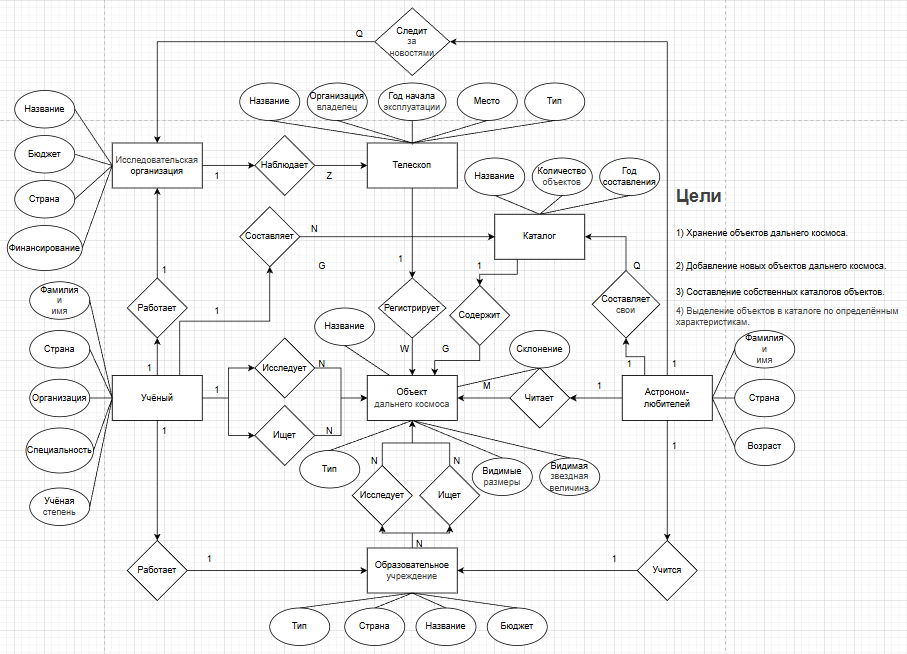
\includegraphics[width=\linewidth,height=\dimexpr\textheight-4\baselineskip\relax,keepaspectratio]{ER.png}
      \caption{ER--диаграмма}
      \label{fig:ER}
    \end{figure}

  \restoregeometry
  \clearpage

        \newpage

        Чтение диаграммы:
        \begin{itemize}
            \item \textbf{Учёный} работает в \textbf{исследовательской организации};

            \item \textbf{Учёный} работает в \textbf{образовательном учреждении};

            \item \textbf{Учёный} исследует \textbf{объект дальнего космоса}

            \item \textbf{Учёный} ищет \textbf{объект дальнего космоса} в каталоге;

            \item \textbf{Образовательное учреждение} исследует \textbf{объект дальнего космоса}

            \item \textbf{Образовательное учреждение} ищет \textbf{объект дальнего космоса};

            \item \textbf{Астроном-любитель} учится в \textbf{образовательном учреждении};

            \item \textbf{Астроном-любитель} составляет свои \textbf{каталоги};

            \item \textbf{Астроном-любитель} следит за новостями об \textbf{исследовательской организации};

            \item \textbf{Исследовательская организация} наблюдает в \textbf{телескоп};

            \item \textbf{Телескоп} регистрирует \textbf{объекты дальнего космоса};

            \item \textbf{Каталог} содержит в себе \textbf{объекты дальнего космоса}.
        \end{itemize}

        \subsection{Иерархическая модель данных}

        Иерархическая модель данных — это способ организации информации в виде древовидной структуры с родительскими и дочерними элементами. Ниже приведена иерархическая модель для данной предметной области (рис. \ref{fig:IE}).

        \begin{figure}[H]
			\centering
			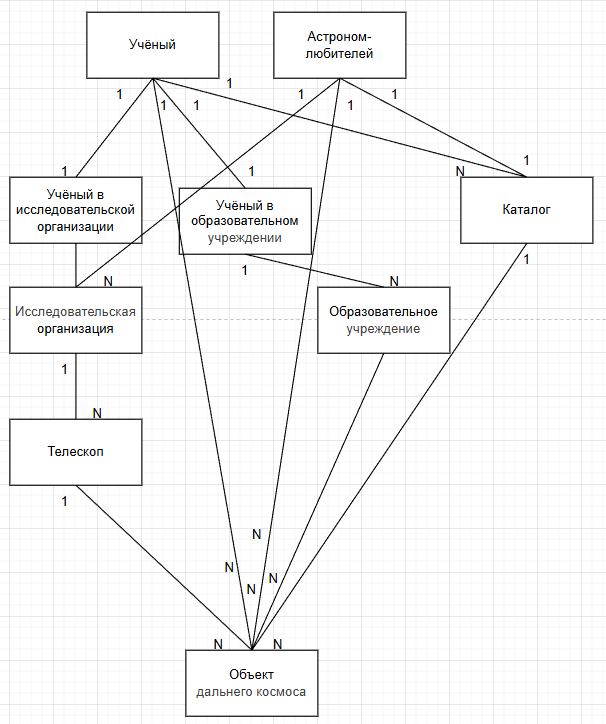
\includegraphics[width=0.85\linewidth]{IE}
			\caption{Иерархическая модель данных.}
			\label{fig:IE}
		\end{figure}
\end{document}